% AUR:
% SHOW THE 2 ATTACK EXAMPLES MENTIONED ABOVE
% (MALICIOUS MAINTAINER AND VCS ATTACK USING SHA1 COLLISION)

% - Bauerbill (detects maintainer changes; allows trusting maintainers globally, for specific packages, or for specific package-timestamp combinations)
% - Aurutils (aursync allows verifying all downloaded build files at once before proceeding with the source download and installation)
\label{sec:eval}
\subsection{Effectiveness of AURsec}\label{sec:security_comparison}
Two notable AUR helpers provide some degree of security: \texttt{aurutils}~\cite{gh:aurutils}, which at least incentivizes users to inspect build files before installing a package, and \texttt{bauerbill}~\cite{bauerbill}, which also provides a local trust management system.
The most common AUR helper, \texttt{yaourt}, disincentivizes users from checking build files because it takes multiple manual steps for each package to do so.

In order to evaluate the performance of \texttt{aursec}, we compared how well it fared against the other two tools in the two attack scenarios that we identified in Section~\ref{sec:attack_scenarios}.

In the scenario from Section~\ref{sec:maint_attack}, the assumption is that a malicious maintainer conducts a targeted attack against an AUR user by temporarily modifying the build files.
\texttt{aurutils} allows users to manually verify build files in bulk using a VIM-style file manager before proceeding, and also shows diffs from the previous version if that is available.
Security-conscious and attentive users may therefore catch the malicious modification --- but only if it is not innocuous enough.
For example, an attacker could change the upstream URL to one that looks equally legitimate (but containing malicious code) and adapt the checksums appropriately, in which case most users wouldn't stand a chance.
In addition to manual verification, \texttt{bauerbill}s trust management system would warn the user if the maintainer of the package changed (such as during adoption of an orphan package), an example of which can be seen in Figure~\ref{fig:bb-query_trust}.
However, if the attack doesn't rely on taking over an orphan package because the existing maintainer is malicious, his SSH key was compromised, or similar, \texttt{bauerbill} doesn't provide more security than \texttt{aurutils}.
\texttt{aursec} easily detects this attack (as long as enough users participate for a useful consensus to have been formed) because the malicious modification would trigger a hash mismatch, of which the user would be warned as seen in Section~\ref{sec:aursec}

\begin{figure}
	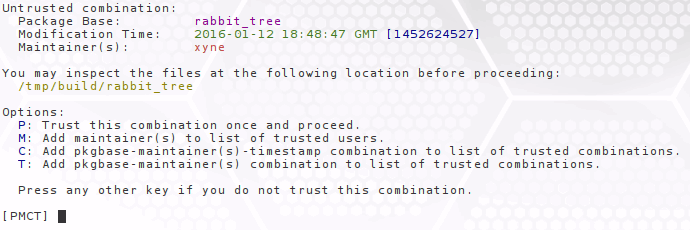
\includegraphics[width=\linewidth]{img/bb-query_trust-screenshot.png}
	\caption{Bauerbills trust management system \cite{bauerbill}}
	\label{fig:bb-query_trust}
\end{figure}

In the scenario from Section~\ref{sec:vcs_attack}, the assumption is that an upstreams VCS repository was attacked or made malicious changes.
No AUR helper is capable of detecting this attack because source integrity verification is normally handled my \texttt{makepkg}. If no checksums are available in the PKGBUILD, such as is the case for VCS packages, nothing can be done with the existing infrastructure.
However, \texttt{aursec} handles this exactly like it handles the previous attack because it hashes VCS sources in addition to the build files.

Therefore, \texttt{aursec} provides superior protection to existing solutions. The comparison is summarized in Table~\ref{tab:defence-comparison}.

\begin{table}
	\centering
	\begin{tabular}{l|m{3cm}|c|m{3cm}}
	\hline

	\hline
	\textbf{Detected Attack} & \textbf{AURsec} & \textbf{Bauerbill} & \textbf{aurutils} \\
	\hline
		Maintainer change & any change without new version & yes & no \\
		Modified build files & yes & manually & manually, diffs between versions \\
		Manipulated VCS sources & yes & no & no \\
	\hline

	\hline
	\end{tabular}
	\caption{Comparison of defence methods against our attack scenarios}
	\label{tab:defence-comparison}
\end{table}

% OTHER PACKAGE MANAGERS:
% EXPLAIN THAT THEY ARE INSECURE AS S**T
% AND THAT OUR APPROACH COULD BE ADAPTED TO THEM,
% allthough not as easily because the AUR has modular helpers already,
% whereas adapting to the other platforms would require forking/patching more monolithic tools or building custom ones

\subsection{Applicability to other packaging systems} % TODO: @lukas better wording instead of "community packaging systems"?
As noted in the introduction, other community packaging systems share security issues with the AUR, which means that most of the analysis from Section~\ref{sec:security_issues} also applies to them.
The \emph{Python Package Index} allows signing of packages with GPG, but its client (\texttt{pip}) cannot verify them~\cite{pypi:security}, so users would need to do that by hand.
There is also no web of trust or any similar mechanism, so users would need to build trust in every individual maintainer.
This is exactly the same situation as that of the AUR.

The \emph{Node package manager} is even worse: There is no means for any signing whatsoever~\cite{npm:security}.

Out of all community package managing systems we looked at, \emph{rubygems.org} is the only one that is open about the state of its security, but they also have the same problems:

\begin{displayquote}
RubyGems has had the ability to cryptographically sign gems since version 0.8.11. This signing works by using the gem cert command to create a key pair, and then packaging signing data inside the gem itself. The gem install command optionally lets you set a security policy, and you can verify the signing key for a gem before you install it.

However, this method of securing gems is not widely used. It requires a number of manual steps on the part of the developer, and there is no well-established chain of trust for gem signing keys. Discussion of new signing models such as X509 and OpenPGP is going on in the rubygems-trust wiki, the RubyGems-Developers list and in IRC.~\cite{rubygems:security}
\end{displayquote}

The communities of the above community packaging systems have been talking about security improvements for years (since about 2012 in most cases), but no significant work has been done to this day.
Since it works purely on the client side and doesn't require any modifications to infrastructure, the solution implemented by AURsec would also be applicable to these other systems.

However, it would take much more work than for the AUR because of the different nature of the ecosystems.
While the AUR is one central location, there is no official client for it, so many users use it by hand and a wide range of (often easily extensible) AUR helpers is available.
This makes it comparatively easy for people to use \texttt{aursec} with their existing workflow.
In contrast, the other community packaging systems each have \emph{one} monolithic official client, and none of them have sufficient hook or plugin mechanisms to make them extensible enough for something like AURsec, so adapting our work to those platforms would require creating custom clients or the distribution of patched versions of the official ones.
